\begin{section}{Resultados}
	El algoritmo de $Newton$ utilizado para buscar los ceros de un polinomio hace uso de dos parámetros, los cuales tuvimos que ajustar de manera de conseguir los mejores resultados posibles, mejores en el sentido de relación calidad de la solución y eficiencia en terminos de tiempo del algoritmo.
	
	Uno de los parámetros es para determinar la máxima cantidad de iteraciones que le permitimos al algoritmo buscar. Para ajustar este parámetro BALABALABNAKABALKABKANSJBFDFKBFKDBC.

	El siguiente gráfico se realizó para ajustar un parámetro ($tolerancia$) del programa que sirve buscar los $ceros$ de un polinomio. Este parámetro se utiliza para decidir si un valor es cero, es decir, cuando es menor a la $tolerancia$ lo consideramos cero.
	
	Con esta prueba esperamos ver que cuanto menor es la $tolerancia$ mejor es la aproximación al cero teórico. Recordar que el algoritmo que busca los ceros de un polinomio tiene dos criterios de parada (la tolerancia y la cantidad de iteraciones permitidas), creemos que la aproximación va a mejorar al disminuir la tolerancia ya que si termina por el primer motivo el valor conseguido va a ser más refinado (más cercano a 0) y si lo hace por el segundo va a mejorar la aproximación durante más iteraciones.\\
	
	Para poder analizar si existen diferencias en el uso de distintas parametrizaciones se creó un generador de puntos de control partir de un par de polinomios (uno para la coordenada $x$ y otra para $y$) los cuales forman la curva. Los puntos de control pueden ser elegidos de forma aleatoria o uniforme. Graficamos entonces el polinomio con los puntos de control seleccionados de alguna de las dos formas anteriormente mencionadas, y las curvas utilizando las distintas de parametrizaciones (uniforme, por longitud de cuerda y centripeta).
	
	Los siguientes gráficos utilizan un conjunto de cinco puntos de control aleatorios dada la misma curva.
	
	\begin{figure}[H]
	  \centering
		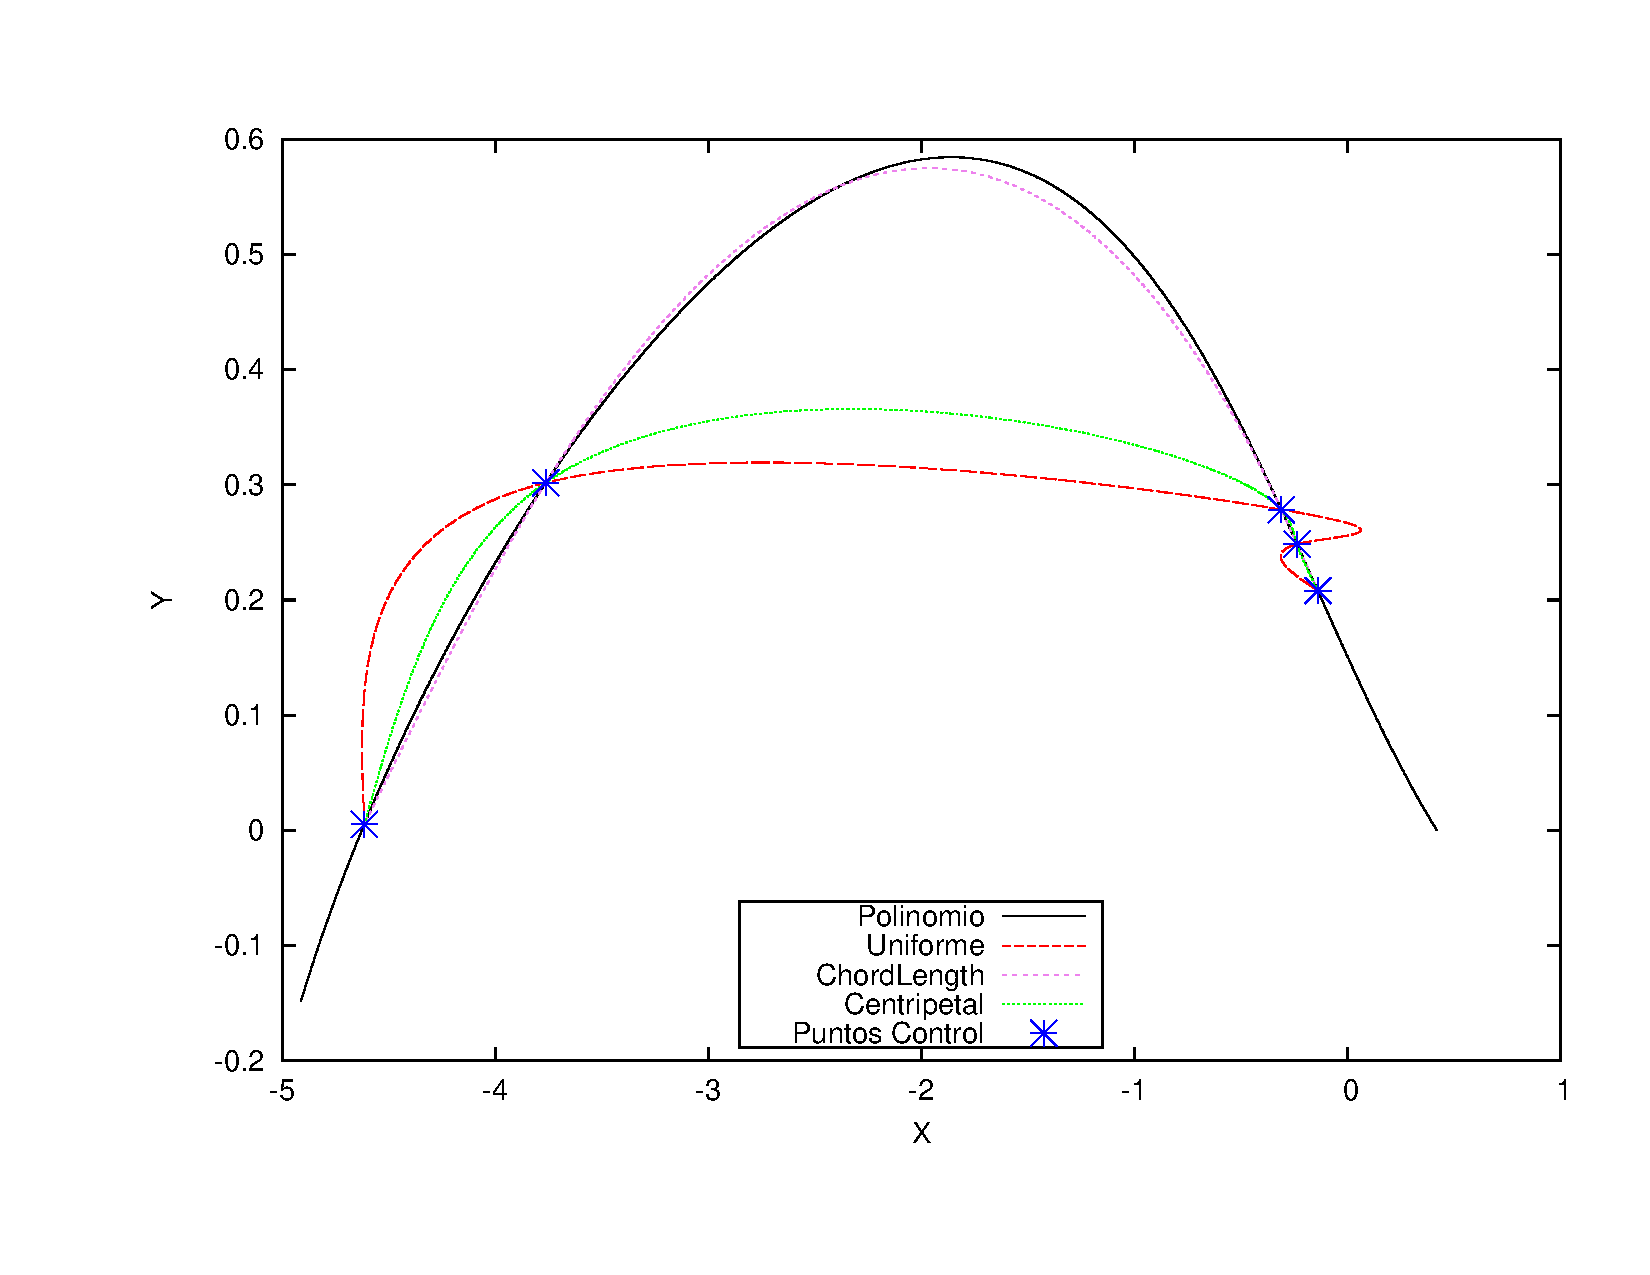
\includegraphics[width=14cm]{graficos/5p_r.pdf}
	  \caption{Aproximación por las distintas parametrizaciones utilizando cinco puntos de control aleatoreos}
	  \label{fig:5p_r}
	\end{figure}
	
	\VSP
	
	
	\begin{figure}[H]
	  \centering
		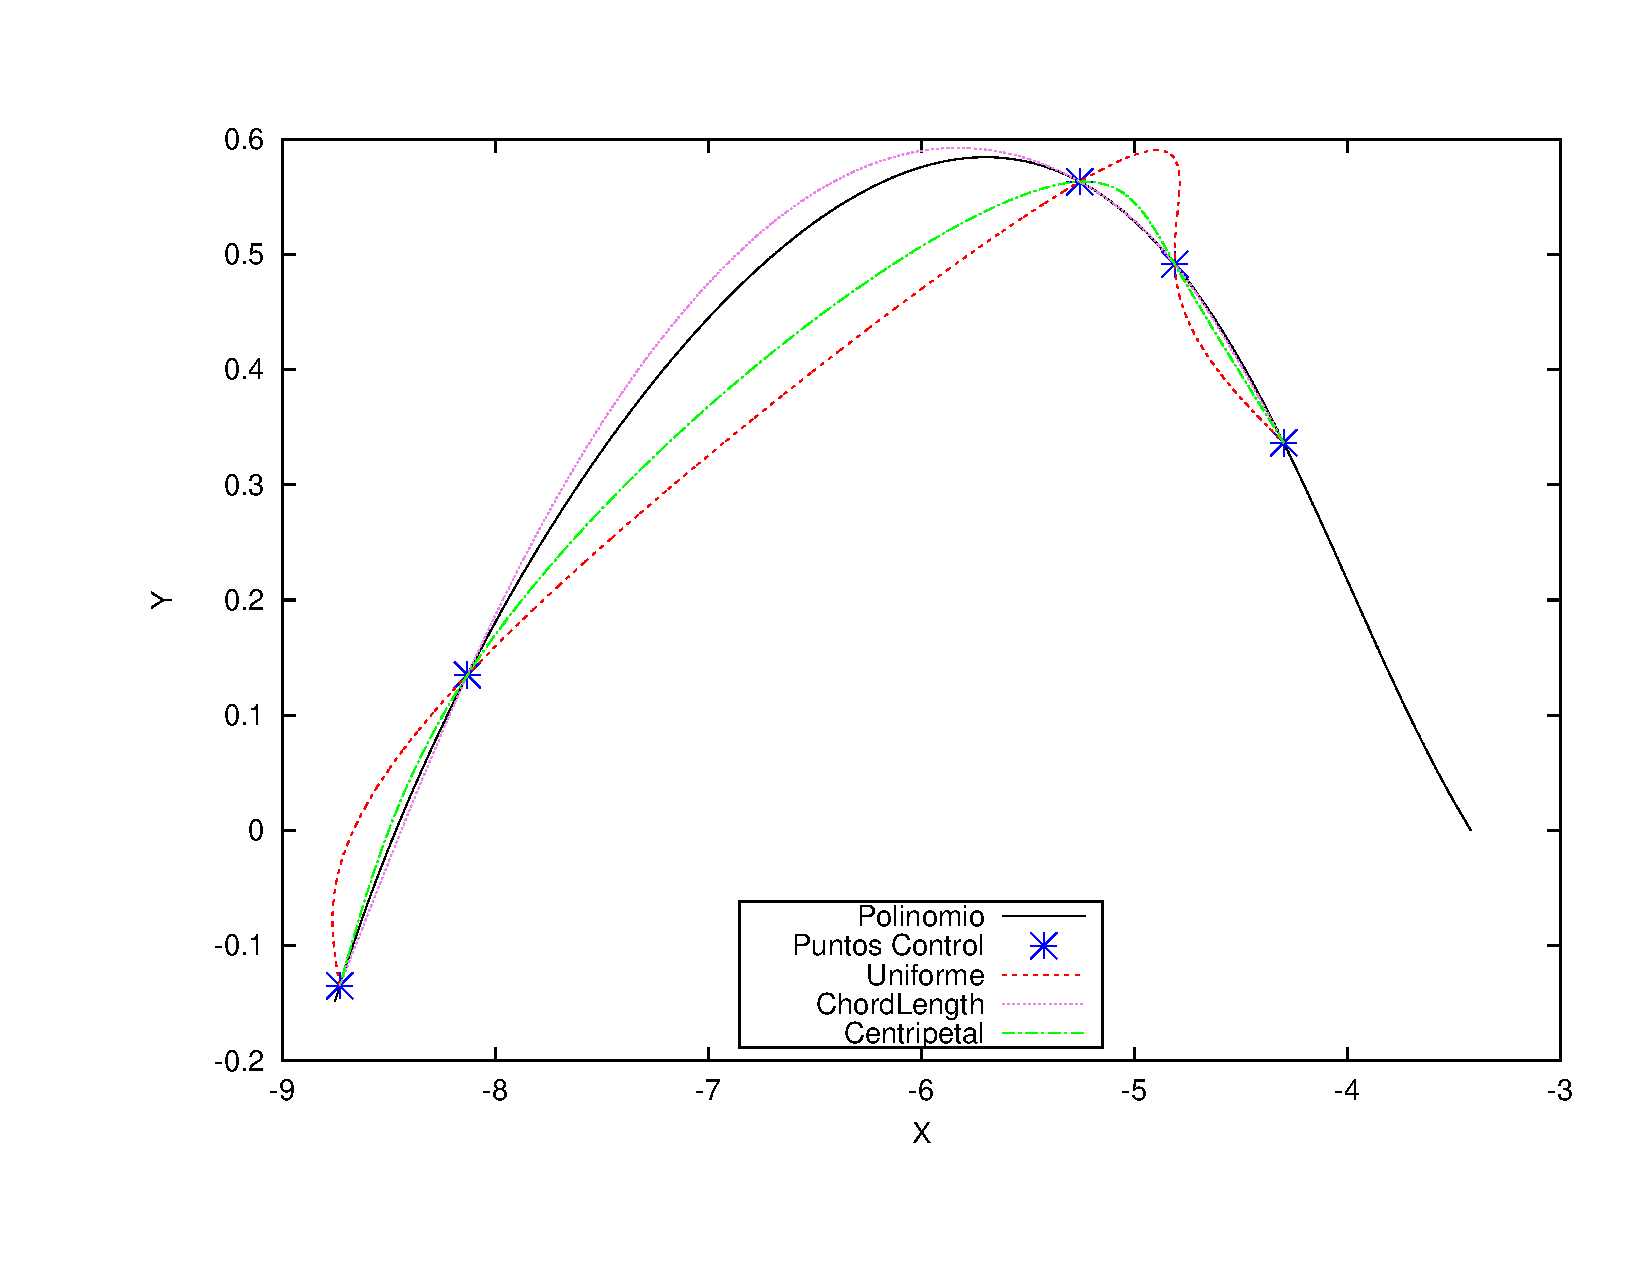
\includegraphics[width=14cm]{graficos/5p.pdf}
	  \caption{Aproximación por las distintas parametrizaciones utilizando cinco puntos de control aleatoreos}
	  \label{fig:5p}
	\end{figure}
	
	\VSP
	
	A continuación, se utiliza el mismo polinomio que el gráfico anterior pero tomando los puntos de control uniformemente.
	
	\begin{figure}[H]
	  \centering
		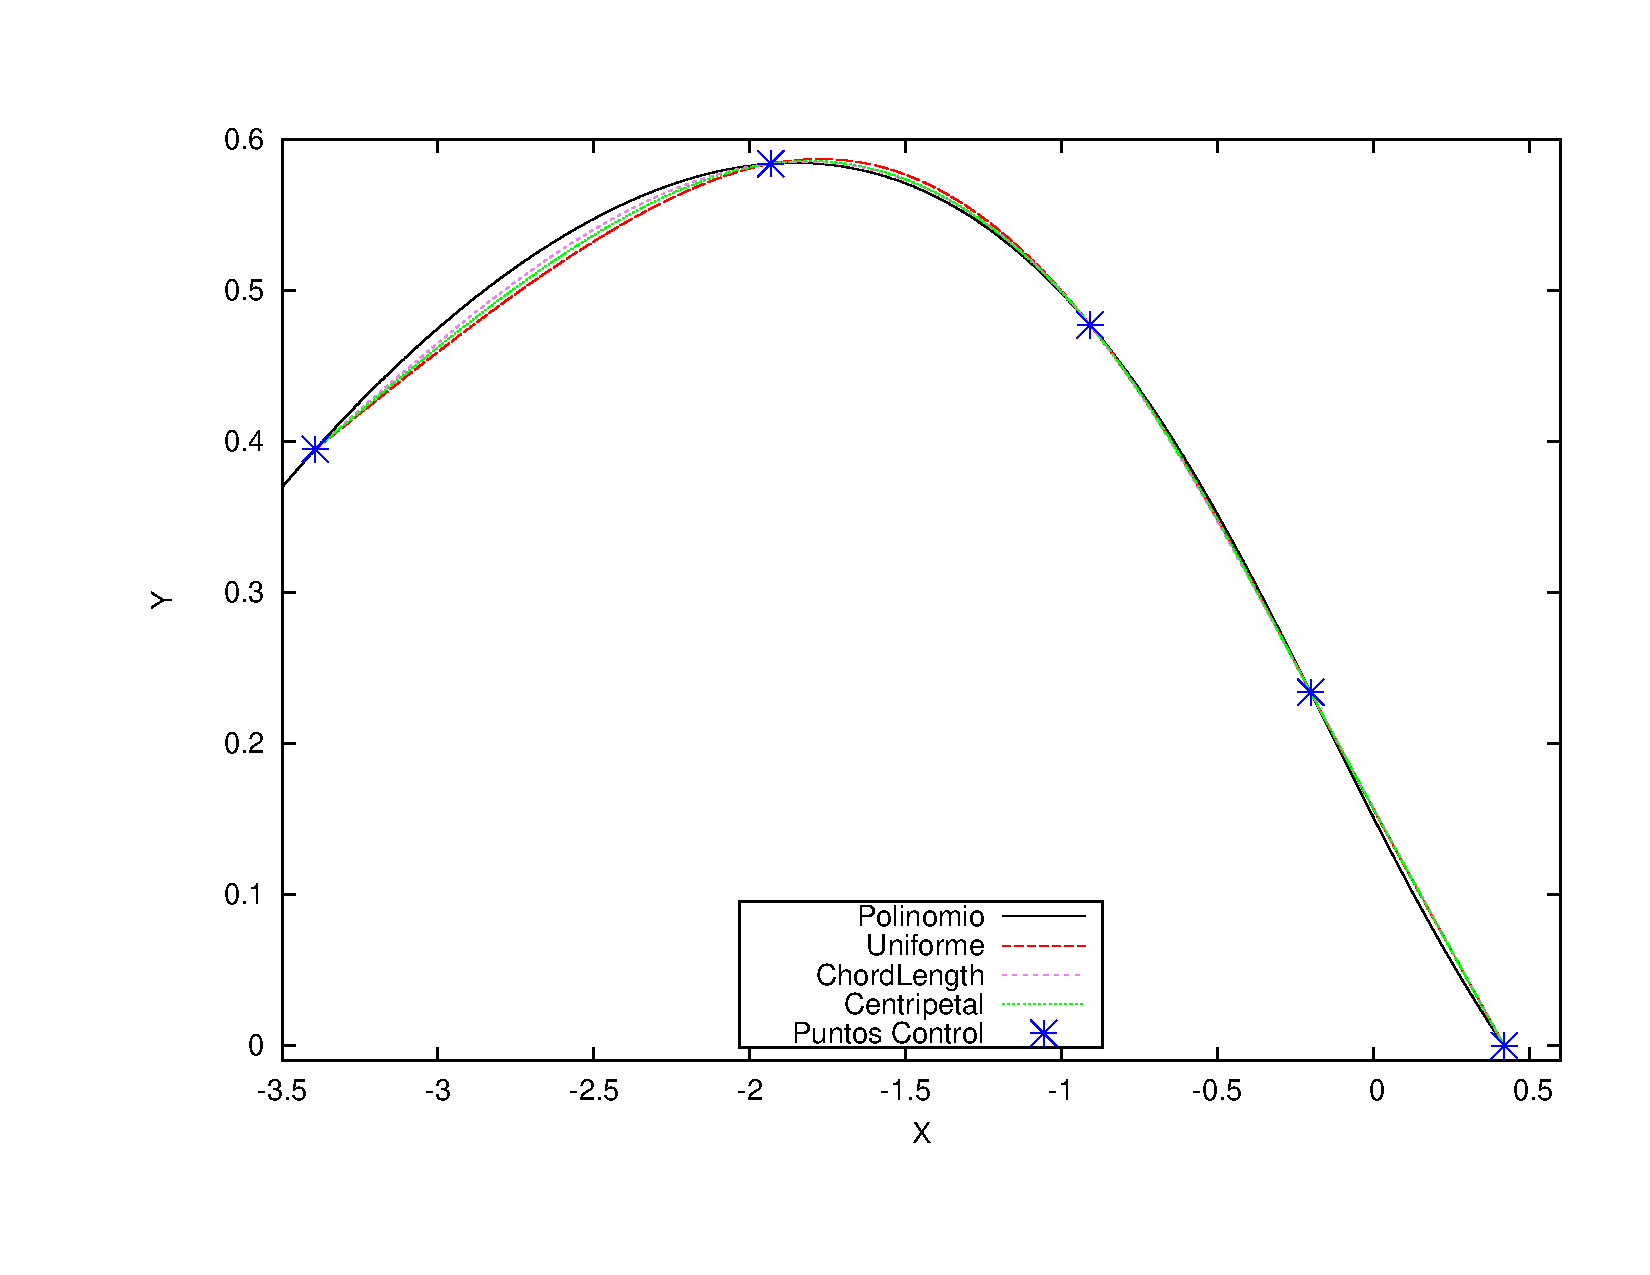
\includegraphics[width=14cm]{graficos/5p_u.pdf}
	  \caption{Aproximación por las distintas parametrizaciones utilizando cinco puntos distribuidos uniformemente}
	  \label{fig:5p_u}
	\end{figure}
	
	\VSP

	Los siguientes gráficos detallan cómo cambia la aproximación a una curva dada una parametrización a medida que existen más puntos de control. Los puntos fueron tomados aleatoreamente y se utilizó la misma curva para las tres parametrizaciones para una comparación y análisis más claro.
		
	El primero de los gráficos muestra la variación en la aproximación dada la parametrización uniforme.
		
	\begin{figure}[H]
	  \centering
		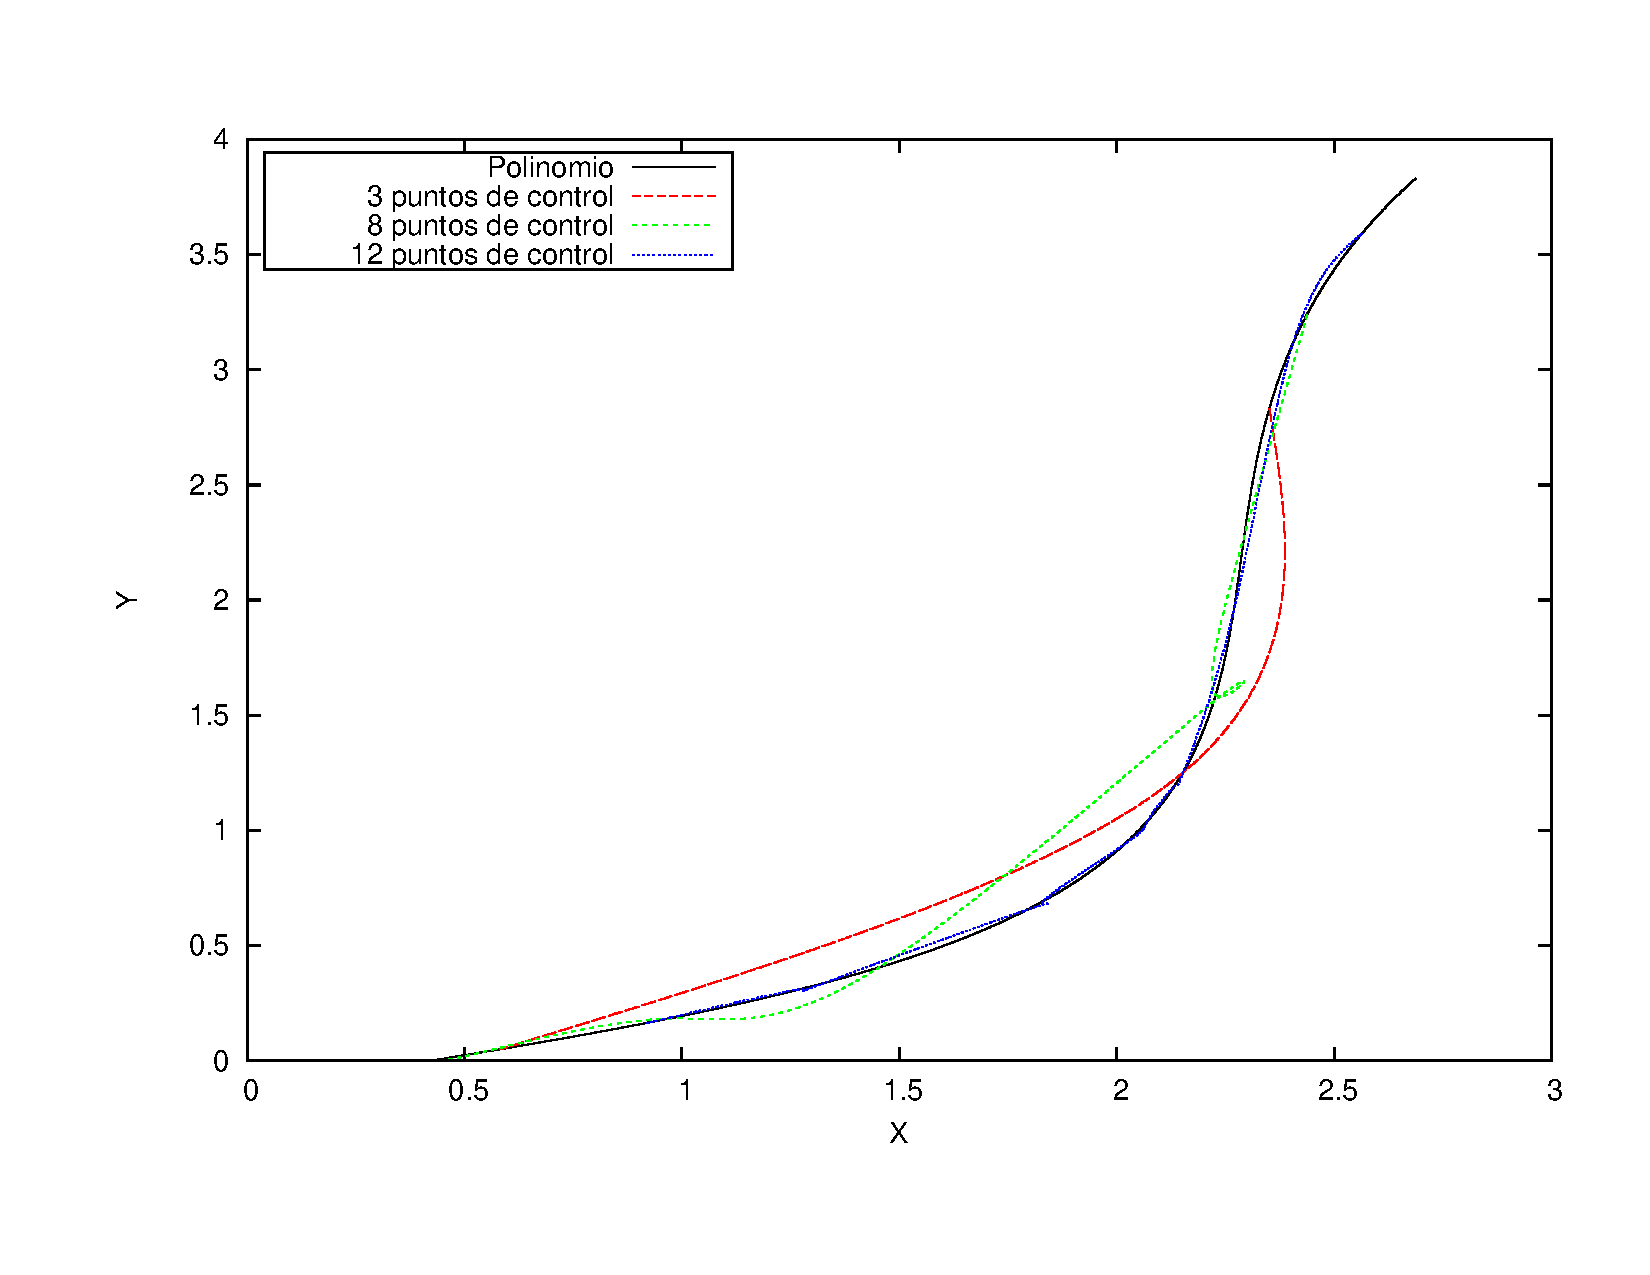
\includegraphics[width=14cm]{graficos/uniform_grafiquinSame.pdf}
	  \caption{Aproximación utilizando parametrización uniforme}
	  \label{fig:uniform}
	\end{figure}
	
	\VSP
	
	Aproximación dada la parametrización centrípeta.
	
	\begin{figure}[H]
	  \centering
		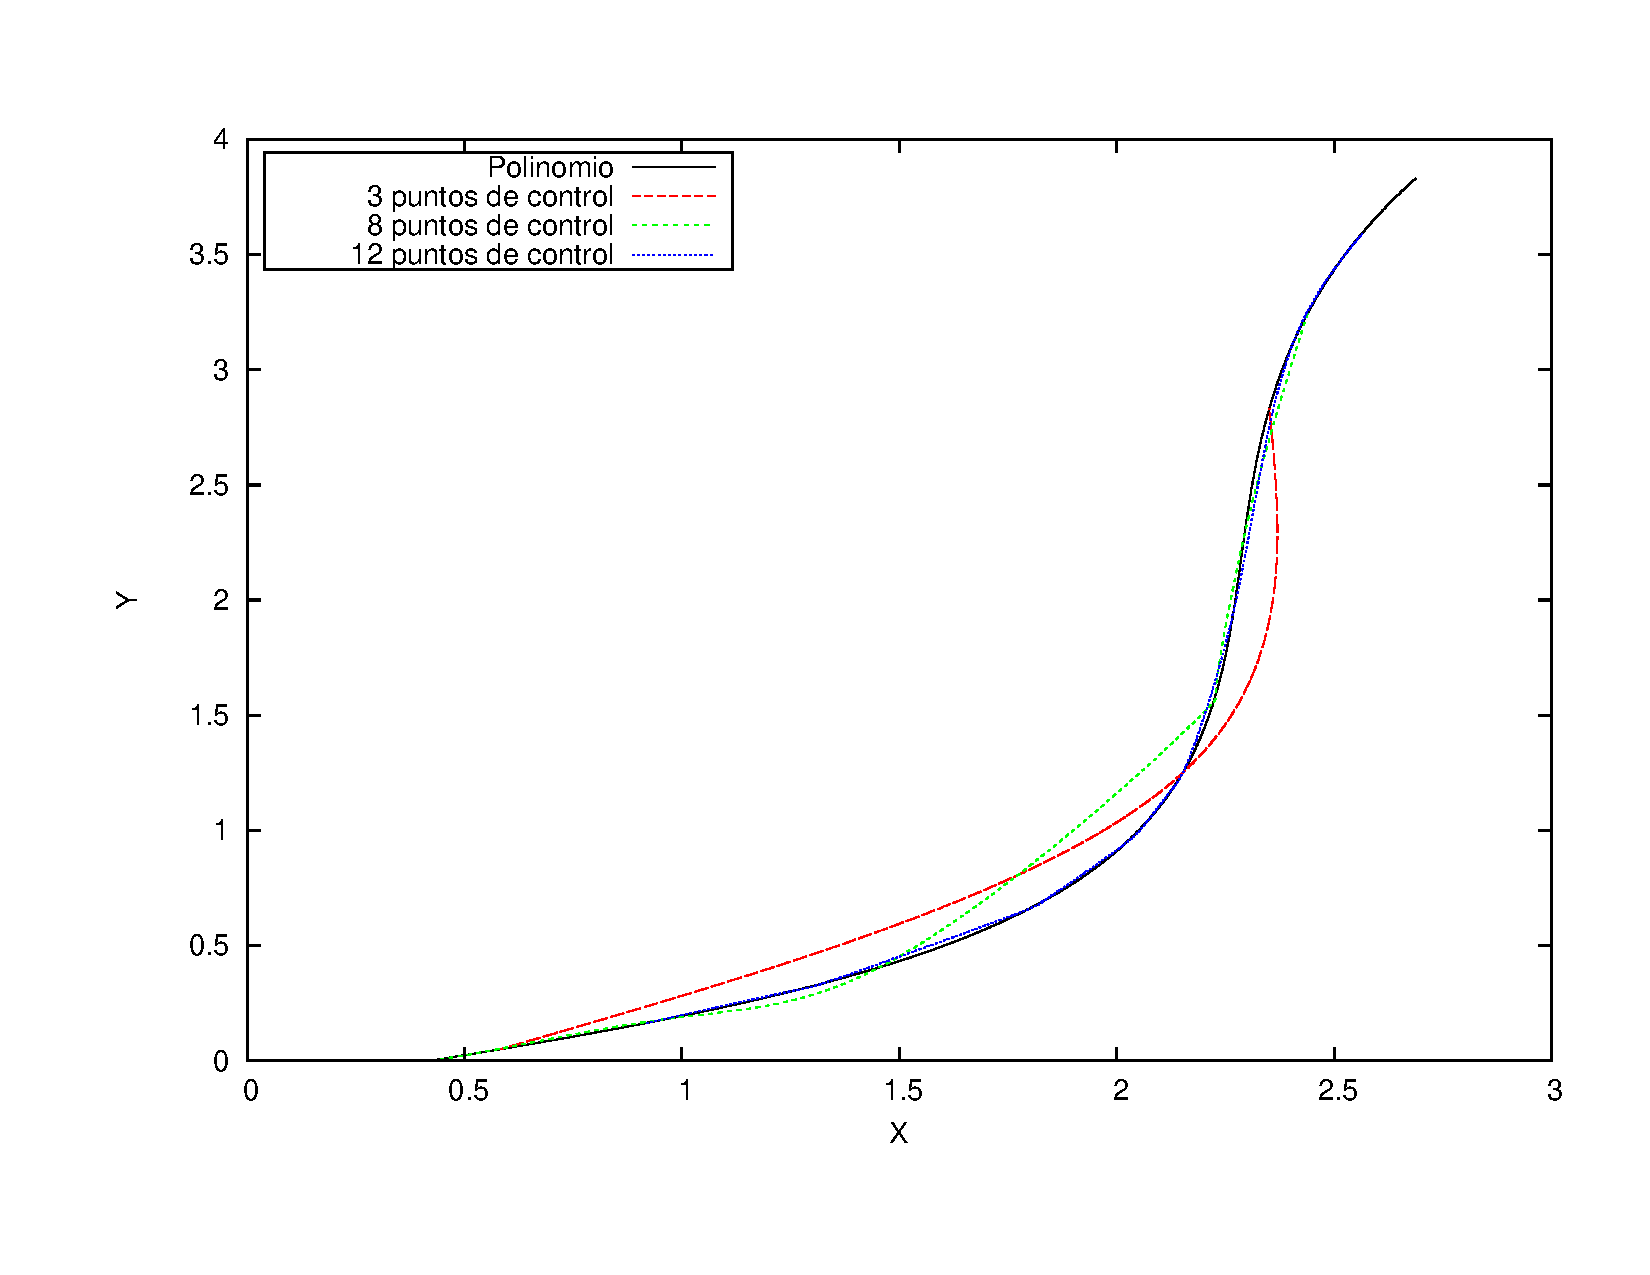
\includegraphics[width=14cm]{graficos/centripetal_grafiquinSame.pdf}
	  \caption{Aproximación utilizando parametrización centrípeta}
	  \label{fig:centripetal}
	\end{figure}
	
	\VSP

	Gráfico utilizando parametrización por longitud de cuerda.

	\begin{figure}[H]
	  \centering
		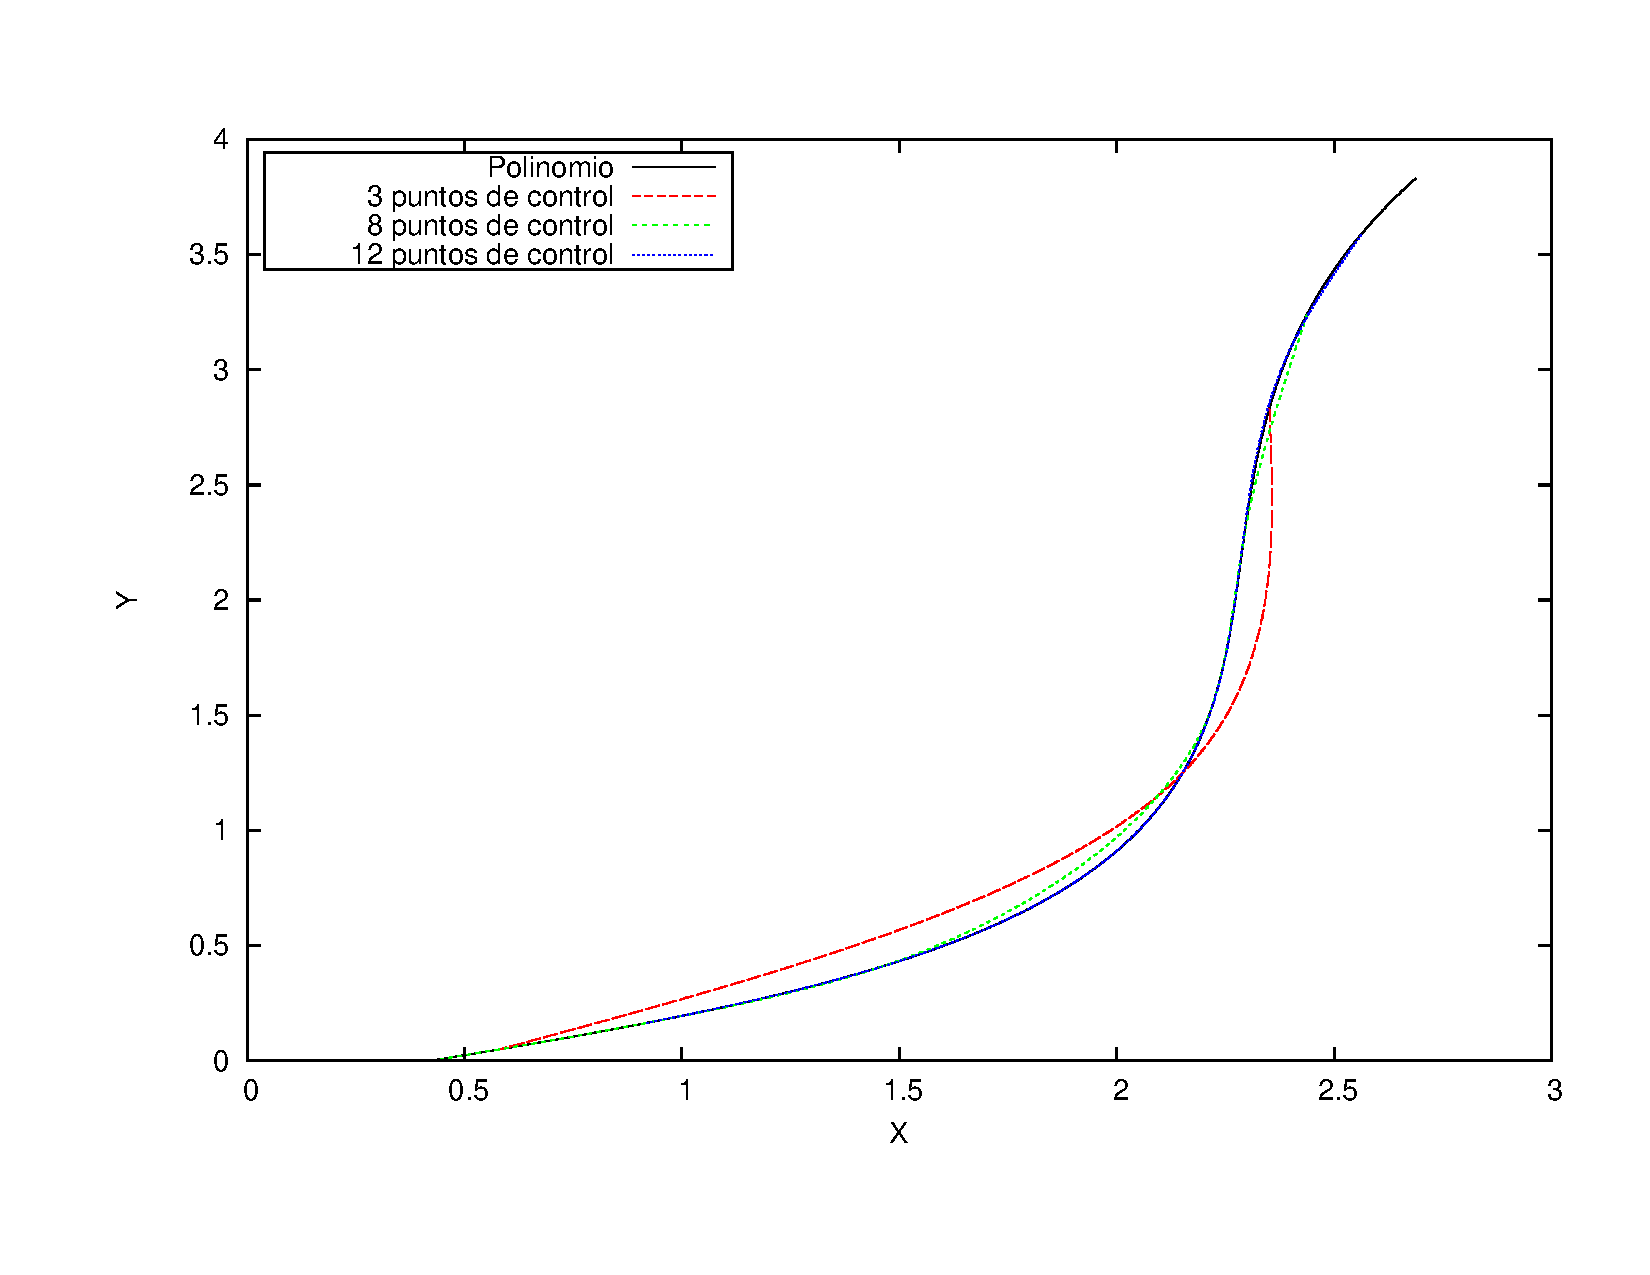
\includegraphics[width=14cm]{graficos/chordLength_grafiquinSame.pdf}
	  \caption{Aproximación utilizando parametrización por longitud de cuerda}
	  \label{fig:chordLength}
	\end{figure}
	
	\VSP
	

	
\end{section}
